\documentclass[a4paper, 11pt]{article}
\usepackage[utf8]{inputenc}
\usepackage{float}
\usepackage{graphicx}
\usepackage{url}
\usepackage{enumitem}
\usepackage{subcaption}

\setlist[itemize]{itemsep=0.5pt, parsep=0.5pt, topsep=0pt, partopsep=0pt}
\setlist[enumerate]{itemsep=0.5pt, parsep=0.5pt, topsep=0pt, partopsep=0pt}

%opening
\title{HW2 Report, Rudy: A Small Routing Protocol}
\author{David Fischer}
\date{\today{}}

\begin{document}

\maketitle

\section{Introduction}
The link-state routing protocol is a key factor enabling the modern internet. OSPF (Open Shortest Path First) is one of the most widely deployed link-state protocols, running in enterprise environment and used by ISPs (Internet Service Providers.)

As part of this assignment \textit{Routy}, a small routing protocol implementing link-state was implemented. 
The routers, or Erlang processes, are able to build a routing table using the Dijkstra algorithm, send messages and share link-state information with other routers using \textit{signals}, and communicate over different machines.

\section{Main problems and solutions}

\subsection{Module Based Approach}

The primary challenge this assignment presented was the module based approach, building up five modules with little correlation made it difficult to see a bigger picture early on. 

To overcome this and prevent any tech debt from building up from incorrect module implementations, a set of tests was created based on the assignments given test commands to ensure proper functionality before moving on to the next module.
The purpose of each module became immediately clear after building the main router implementation, tying together all of the modules and observing their behavior in the complete system solidified the understanding of the entire stack. 

\subsection{Debugging Final Implementation}

Debugging the final implementation did present challenges primarily with the traceability of calls in a distributed system. With five modules and more than three processes running at a time, reading and correctly understanding the diluted log output was troublesome.

This was solved by ensuring a structured log output, debugging single modules and removing log output from any unrelated components to reduce noise, and automating test cases.

\subsection{Duplicate Update and Broadcast}

The issue the most time was spent on was each router needing \textit{two} broadcast and update cycles to create a complete topology, it was also tackled last since it didn't make any functional difference for testing.

After the debugging methods from the previous section were applied the issues was traced to the \textit{hist} module.
To implement the module, the \textit{Map} data type and \texttt{get(Key, Map, Default) -> Value | Default} were used.
All routers start out with \textit{0} as their initial message number while the \texttt{Default} parameter for the \texttt{get/3} function was also set to \textit{0}.
This resulted in the first message from any router being disregarded as old, since they weren't registered in the map yet, resulting in the first message defaulting to being old. The second message with the number \textit{1} was then interpreted as new.
Additionally, to make routers always interpret their own messages as old, Erlang's type order placing atoms before numbers was applied, setting the nodes own entry to \textit{inf}, thus making any greater than comparison result in \texttt{true}.

\section{Evaluation}

To efficiently evaluate and debug the implementation, a testing module to set up multiple routers, connections, and messaging across different countries, or machines, was created.
Figure \ref{fig:map1} is an approximate illustration of the testing environment including nine routers in Austria and five routers in Germany with directional and bidirectional connections.

This setup proved crucial in confirming functionality and analyzing the behavior of the distributed system, also helping identify many of the nuances of this link-state implementation. 
The most significant learnings came from shutting down individual routers and seeing the Dijkstra algorithm compute new optimal paths going around the outage, or correctly identifying that certain routers are now unreachable through the \texttt{entry/2} function.
This also caused the most interesting edge case when broadcasts and updates aren't propagated through the entire network, leading to infinite message routing loops between two nodes.
This occurs when a router doesn't have an up to date view and tries to communicate over another router which does. In the worst case, the second node has identified the message path to go back over the original router, leading them to continuously send the message back and forth.

\begin{figure}[H]
  \begin{center}
    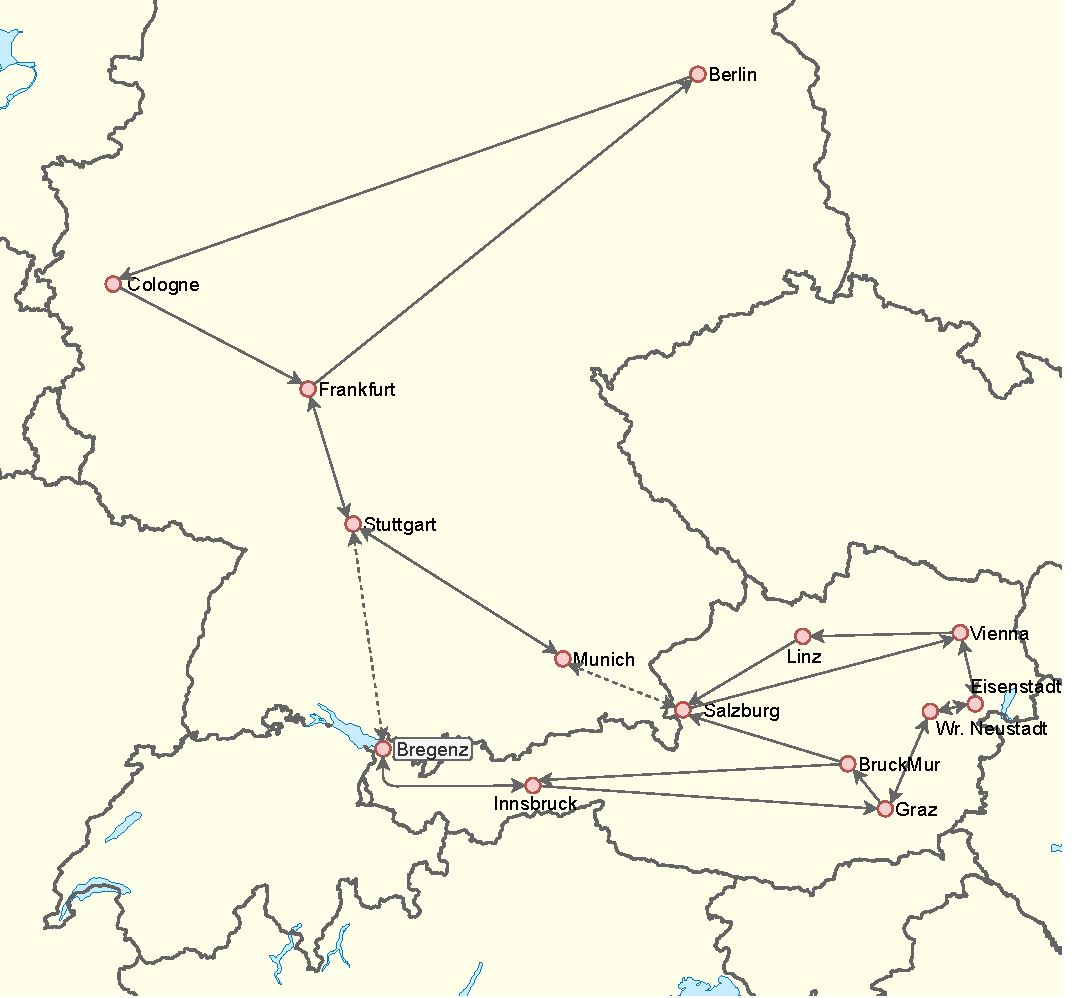
\includegraphics[width=345px]{graphics/map_routy.pdf}
    \caption{Map of routers used for evaluation.}
    \label{fig:map1}
  \end{center}
\end{figure}

% removing routers either through deletion or them going down can cause infinite loops between routers

%  1. salzburg goes down
% 2. vienna detects the 'DOWN' message and removes salzburg from its routing table
% 3. But linz still thinks salzburg exists and has a route to vienna through salzburg
% 4. When you send a message to vienna:
%   - linz routes it to salzburg (which is dead)
%   - The message bounces back or gets lost
%   - Or worse, if there are backup paths, it creates routing loops

\section{Conclusions}

This assignment served as an excellent introduction to the inner workings of link-state protocols.
While the sequentially implemented modules did present some initial challenges and lead to some functions being implemented unconventionally for a functional language, showing the authors object oriented background, seeing messages routed over routers written by other classmates in the "The world" bonus task was gratifying. 
Additionally, the bonus task also reinforced the importance of common interfaces in distributed systems, as any deviation would lead to routers throwing an error or not being able to communicate.

Future development should include automatically and periodically updating and broadcasting each routers links to enable a more seamless operation, a separate logging module to handle log levels and structured output, and reducing the complexity and size of the \texttt{router/6} function in the \textit{routy} module.

\end{document}
